\documentclass[a4paper,12pt, twoside]{article}
%\documentclass[a4paper,12pt, twoside]{book}

\usepackage[papersize={210mm,297mm},tmargin=20mm,bmargin=20mm,lmargin=20mm,rmargin=20mm]{geometry}

\usepackage[utf8]{inputenc}
%https://mirror.hmc.edu/ctan/macros/latex/contrib/babel-contrib/turkish/turkish.pdf
\usepackage[english]{babel}
%\usepackage[T1]{fontenc}

\usepackage{amsmath,amssymb,mathabx}%\for eqref
\usepackage{lscape}
\usepackage{tcolorbox}

\usepackage{hyperref}
\hypersetup{
    colorlinks,
    citecolor=black,
    filecolor=black,
    linkcolor=blue,
    urlcolor=red}
  

%%% \usepackage{svg}
%%% https://tex.stackexchange.com/questions/122871/include-svg-images-with-the-svg-package/129854
\usepackage{graphicx}
\graphicspath{ {./uygulama_figurleri/} }

\usepackage[colorinlistoftodos]{todonotes}
\usepackage{fancyhdr}

\usepackage{indentfirst}
%% paragraf girintisi
\setlength{\parindent}{5ex}

%% Daha sonra yazılacak kısımları not düşmek için...
\newcommand{\YAZILACAK}{{\vspace{18pt}\bf\Large \color{red} YAZILACAK}}


\pagestyle{fancy}
\fancyhf{}
\lhead{ Kuantum Fiziği - Uygulamalar}
\chead{\thepage}
\rhead{Mesut Karakoç}
\lfoot{Akdeniz Üniversitesi}
\cfoot{}
%\rfoot{BF}

\title{Kuantum Fiziği Ders Notları \\ $\sim$Uygulamalar$\sim$}

\author{\setlength{\unitlength}{6mm}
\begin{picture}(10,10)
	%% picture taken from:
	%% https://www.pxfuel.com/en/free-photo-qauqe
\put(-3.4,0){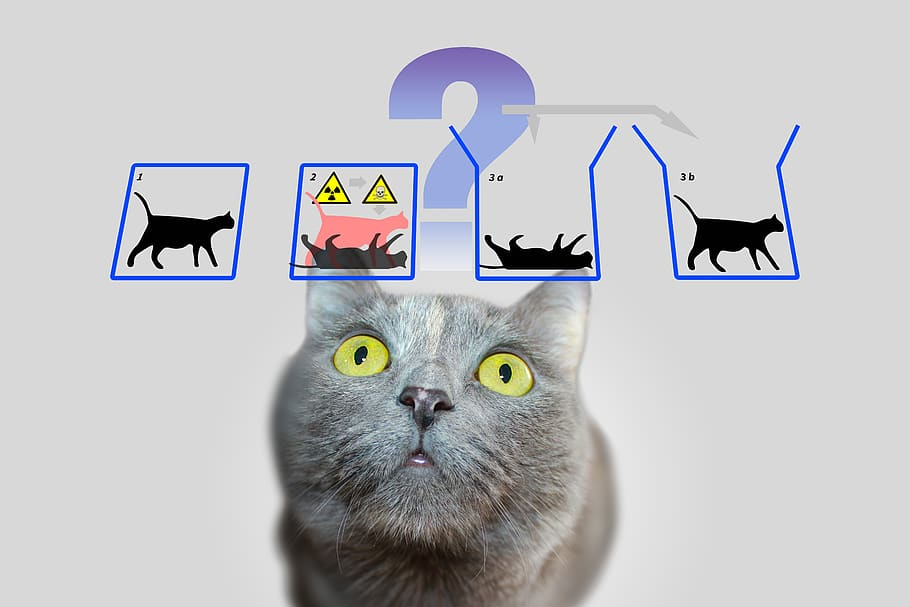
\includegraphics[width=10cm]{physics-schrodinger-s-cat-schrodinger-quantum-mechanics.jpg}}
\end{picture} \\ Doç. Dr. Mesut Karakoç}


\date{\today}

\begin{document}

%% Turkish babel problem
%% https://tex.stackexchange.com/questions/160385/newgeometry-doesnt-work-with-turkish-babel-package
%%\shorthandoff{=}% Make = not active any more

\maketitle

% \newpage
% 
% % change name to "İçindekiler"
% \renewcommand{\contentsname}{İçindekiler}
% \tableofcontents{}
% 
% \listoffigures
%  
% \listoftables

\newpage

\section{Uygulama: 1nci Bölüm}

\begin{enumerate}
	
	\item  Güneşin siyah bir cisim olarak ışıma yaptığını varsayalım. Güneşin yarıçapı $7 \times 10^{8} \mathrm{~m}$ olduğuna göre, (a) saniyede yayılan toplam radyasyon miktarı nedir? (b) Dünya ile güneş arasındaki mesafenin 1,5 $ \times 10^{11} \mathrm{~m}$ olduğu göz önüne alındığında, dünya üzerinde güneş yönüne dik olan $1 \mathrm{~m}^{2}$'lik bir yüzeye ne kadar enerji düşer?  Denklemler (1-1) ve (1-7)'yi kullanabilirsiniz ve güneş yüzeyinin sıcaklığının 6000 $\mathrm{~K}$ olduğunu varsayabilirsiniz.
	
	%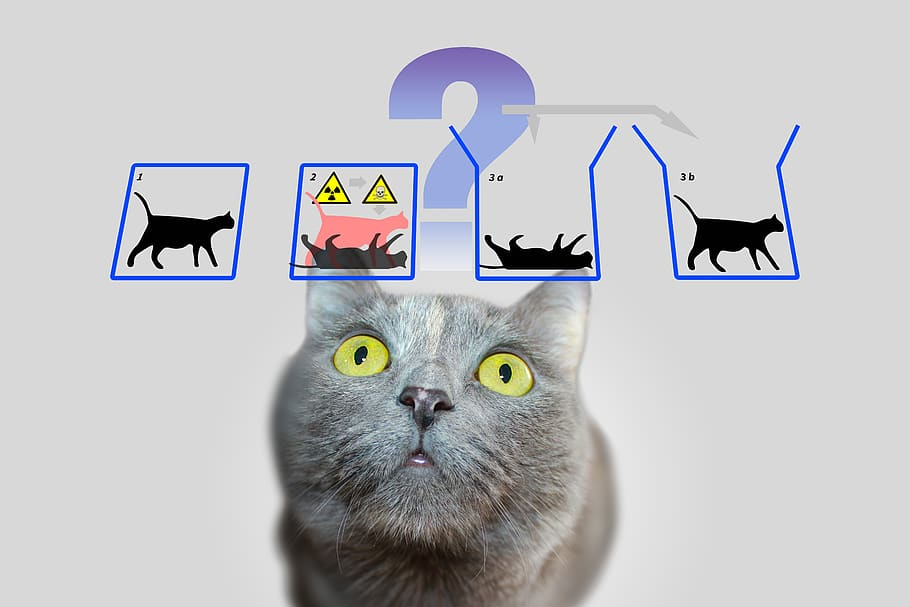
\includegraphics[width=\textwidth]{physics-schrodinger-s-cat-schrodinger-quantum-mechanics.jpg}

	{\bf Çözüm:} Sırasıyla denklem (1-1) ve (1-7) aşağıda verilmiştir.
	\begin{align}
		\omega(\lambda, T) &=\frac{4}{c} E\left(\lambda, T\right) \\
		U(T) &=\int_{0}^{\infty} \omega(\lambda, T) d \lambda =\int_{0}^{\infty} u(\nu, T) d \nu=a T^{4}
	\end{align}
  
    

	\begin{align}
		E(T) =\int_{0}^{\infty} E(\lambda, T) d \lambda = \sigma T^{4}
	\end{align}

    


	
	\item Stefan-Boltzmann yasasındaki a sabiti için boyut analizini kullanarak $h$ (Planck sabiti) ve $c$ (ışık hızı) cinsinden bir ifade yazınız.
	
\end{enumerate}

\end{document}

